Accurate interatomic potentials are essential for applications in chemistry, molecular biology, and material sciences. At the lowest level, it is possible to solve these many-body systems \textit{ab initio} using a simulation of Schr\"odinger's equation, though this is not computationally feasible at even small scales due to the exponential growth of the Hilbert space, therefore different alternatives have been devised at various levels of the speed vs. accuracy trade off. Treating all charges as points, we achieve the many-body expansion see in Equation \ref{eq:interatomic-potential}. Again, in larger systems calculations quickly become intractable due to the number of terms growing combinatorially with body-order. Density Functional Theory (DFT) \cite{hohenberg1964inhomogeneous, kohn1965self} has long been the antidote to this poor scaling by offering an extremely accurate, tractable framework to calculate interatomic potentials. Although much faster than using Equation \ref{eq:interatomic-potential}, DFT still takes $\sim10^3\mathrm s$ for small molecules of $\sim 20$ atoms and on the order of days for larger molecules.


\begin{equation} \label{eq:interatomic-potential}
    E_i = E^{(1)}(\mathbf r_i) + \frac 1 {2}\sum_{j}E^{(2)}(\mathbf r_i, \mathbf r_j) + \frac 1 {6}\sum_{j,k}E^{(3)}(\mathbf r_i, \mathbf r_j, \mathbf r_k) + \frac 1 {24}\sum_{j,k,l}E^{(4)}(\mathbf r_i, \mathbf r_j, \mathbf r_k, \mathbf r_l) + \cdots
\end{equation}

Machine Learning Interatomic Potentials (MLIP) emerged from the desire to gain more speed improvements while retaining DFT-level accuracy. Where DFT uses input positions and a computational method derived from physics to calculate output properties, MLIPs use input positions and training data from DFT to reconstruct a new computational method that approximates the original that is run at a fraction of the cost. After training, MLIPs are  much quicker as DFT calculations scale cubically with the number of electrons whereas MLIPs often scale linearly with the number of atoms. Machine Learning models are trained by optimising the performance of a function, $f(x_i, w) = y_{i,\text{pred}}$ that predicts the output $y_{i,\text{true}}$ for the input $x_i$. We do this via minimising a loss function, such as the mean square error as seen in Equation \ref{eq:loss}. 

\begin{equation} \label{eq:loss}
    \mathrm{loss} = \mathrm{mean}((y_{i,\text{pred}} - y_{i,\text{true}})^2) = \mathrm{mean}((f(x_i,w) - y_{i,\text{true}})^2)
\end{equation}

For simple models such as linear regression, it is possible to minimise the loss with respect to the parameters analytically via matrix inversion \cite{weisstein2002moore}. In the case of non-linear models such as neural networks, finding an analytical solution is not possible. Equation \ref{eq:grad-desc} shows how these models employ gradient descent to adjust the parameters \textit{a little bit} (the learning rate $\eta$ decides how big this is) in the parameter-space direction that minimises the loss the most. Following each adjustment, the loss is reassessed to determine the new optimal direction for the subsequent parameter shift. In recent years, many physically-inspired additions have been made to this algorithm such as the addition of `momentum' in Adam \cite{kingma2014adam}.

\begin{equation} \label{eq:grad-desc}
 w_{i+1} = w_i - \eta \frac{\partial \mathrm{loss}}{\partial w_i}
\end{equation}

% For our task, we are especially interested in SO(3), the
% group of rotations of R
% 3
% . In fact, 3D symmetries are intertwined with the law of physics describing quantum interactions, i.e. the Schrodinger equations (Schrodinger ¨ , 1926).
% Specifically, if we rotate a system the energy should not
% vary, SO(3)-invariance, and forces should rotate accordingly, SO(3)-equivariance.

% Despite the rigid structure of molecules with their benzene rings, rules for bonding, and *** this does not quite transfer over to $1$s and $0$s of computers - therefore we consider this data unstructured. In principle, it would be possible to turn molecules into images based on their positions and then use canonical computer vision architectures which carry out operations \textit{pixelwise}. Though looking at figure \ref{fig:embed} we see that only 12 of the 196 total pixels are part of the molecule, so most of the time the architecture would be acting on empty pixels i.e. thin air! This would then allow us to carry out operations \textit{nodewise} ensuring that every action of the architecture is actually doing something. 

% need to write here that the graph was not the molecule


Some MLIPs use Basis Function Regression, a type of linear regression that produces a hyperplane of best fit by finding the coefficients to a linear combination of basis functions of variables such as position, atom type etc. An example in 1D is the polynomial set of basis functions (see Equation \ref{eq:basis-func}) which is able to  approximate any continuous function to arbitrary accuracy i.e. is complete.

\begin{equation} \label{eq:basis-func}
    y = \sum_n^\infty \alpha_n x^n = \alpha_0 + \alpha_1 x + \alpha_2 x^2 + \cdots 
\end{equation}

Basis function selection needs to problem specific so is often a process informed by domain knowledge i.e. symmetries, physical laws etc. - the design of models to capture this domain knowledge is referred to as \textit{inductive bias}. Inductive bias restricts the possible function space by not allowing functions that don't obey the symmetry/physical law and therefore reduces the amount of data needed to train 

Over the past decade, many ways have been proposed to find these basis functions \cite{behler2011atom, shapeev2016moment, caro2019optimizing} but this has lacked the clarity of a unified framework which exist for similar problems in adjacent fields such as computer vision \cite{uhrin2021through}. The Atomic Cluster Expansion (ACE) \cite{drautz2019atomic, dusson2022atomic} bridges this gap by offering a treatise in systematically creating sets of basis functions which are provably complete and allows for arbitrarily high-body order at constant cost. It has been shown that many atomic environment descriptors such as MTP, SOAP \cite{shapeev2016moment, caro2019optimizing} can be expressed in the ACE framework. Using these basis states as a basis for basis function regression has proved very effective and rivalled results of many far more complex architectures \cite{kovacs2021linear}.

% what is the deal with ACE here -> about invariants vs. equivariants



% In ACE, a graph structure is formed letting atoms equal nodes and joining atom within some cutoff distance, $r_c$, with edges. This is used in place of the more natural bonds $\equiv$ edges as this misses out non-bonded atoms that are close and effect each other. For each node, its edges are given particle basis states, with are two-body (central and peripheral node) which are aggregated to form an atomic basis (one per node). These atomic basis states can then be multiplied/tensor producted together $v$ times to give $v+1$-body order terms, which form the basis functions $\mathbf{B}$. Using these basis states as a basis for linear regression has proved very effective and rivalled results of many far more complex architectures \cite{kovacs2021linear}.

% maybe here have the thing about how these can approximate equation 1 ?!

At the same time, the deep learning community was tackling MLIPs from a Graph Neural Network (GNN) perspective. Again, nodes share an edge if they are within some cutoff radius, $r_c$. GNNs use one/many rounds of message-passing in which nodes, which carry a list of scalar features, will received `messages' from nodes they share an edge with (their neighbourhood, $\mathcal N$) as a function of these features. These messages are then aggregated in some permutation-invariant (e.g. sum) way and used alongside the current node features as an input to an update function which outputs the new features. Early architectures of this type started off with layers using two-body scalar (i.e. invariant) properties such as relative distance between neighbours \cite{gilmer2017neural, schutt2017schnet}. Other architectures \cite{gasteiger2020directional, liu2021spherical, gasteiger2021gemnet} extended this idea by explicitly forming many-body invariants such as bond angles from the three body terms (in Figure \ref{fig:angles} for nodes $A,C$ in the neighbourhood of $B$: $\vec x_{BA} \cdot \vec x _{BC} \sim \cos \theta_{ABC}$) in DimeNet. These methods offered state-of-the-art results whilst having an inference time $\sim 5$ orders of magnitude less than DFT. As the many-body terms are calculated explicitly these models are subject to the many-body scaling of Equation \ref{eq:interatomic-potential}.

\begin{figure}[H]
    \centering
    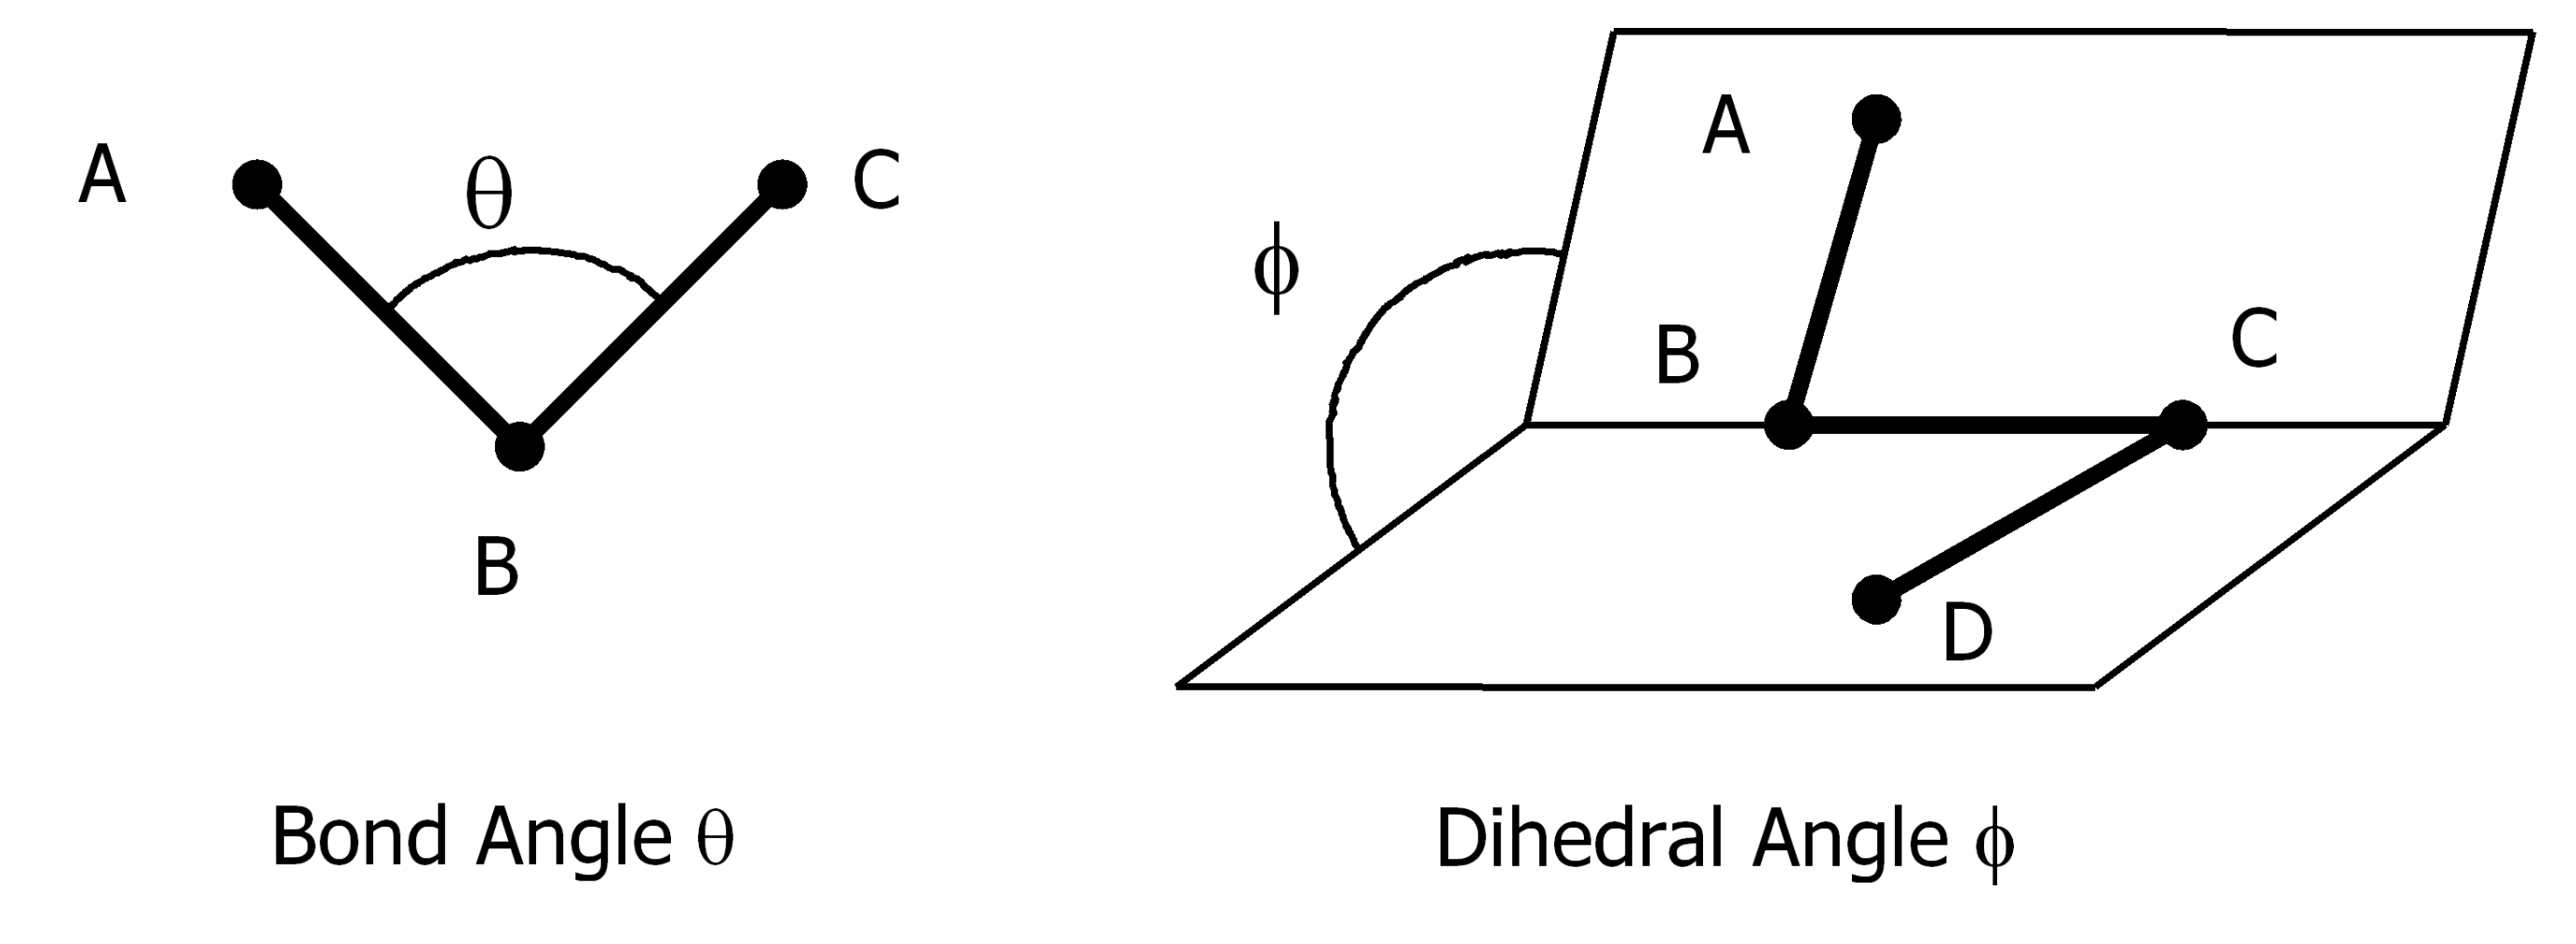
\includegraphics[width=0.7\textwidth]{figures/angles.png}
    \caption{\textit{left}: the angle $\theta$ is a three-body term, as positions of $A, B, C$ are required to calculate via $\vec x_{BA} \cdot \vec x _{BC} \sim \cos \theta_{ABC}$. Note that both vectors $\vec x _{AC}, \vec x _{AC}$ can be generated in the neighbourhood of $B$.\\\textit{right}: the dihedral angle is a four-body term $\vec x_{AB} \cdot \vec x_{CD} \sim \cos \phi$. As these two vectors are from different graph neighbourhoods $\phi$ can only be calculate if vectors are passed between layers. \cite{chemHope2023}}
    \label{fig:angles}
\end{figure}

Invariant scalar features in GNNs can be promoted to equivariant tensors e.g. vectors and matrices. This is on the intuition that equivariant features retain information about the coordinate system between layers which allows for the formation invariants involving geometric properties from multiple neighbourhoods i.e. dihedral angle as seen in Figure \ref{fig:angles}. Also, many physical properties of molecules are non-scalars such as vector dipole moments or polarisability matrices so its good to have features that transform in the same way. This led to the development of many equivariant architectures such as TFN, Comorant, $\mathrm E(n)$-GNN \cite{thomas2018tensor, anderson2019cormorant, satorras2021n}. Though these architectures were brilliant for propagating symmetries through multiple layers, only two-body terms were within a layer so these architectures struggled with some tasks that `simpler' architectures such as Dimenet could solve. Figure \ref{fig:map-timeline}b shows the timeline of both the invariant and equivariant architectures. 

\begin{figure}[H] % at in our contributions here
    \centering
    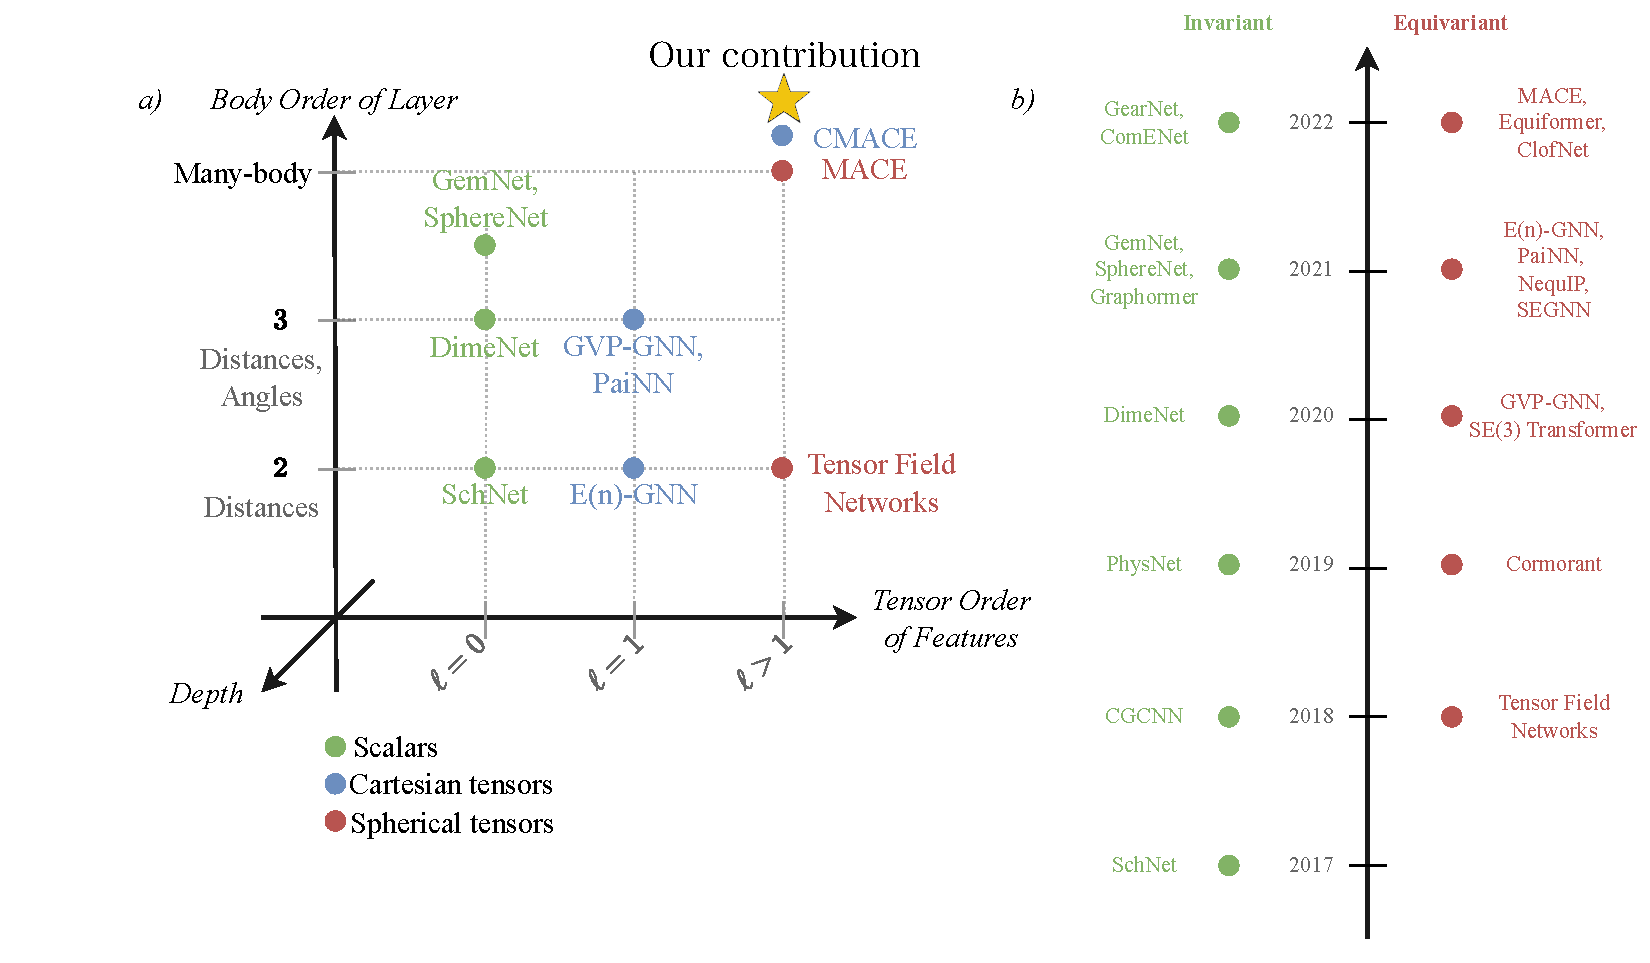
\includegraphics[width=\textwidth]{figures/map-timeline.pdf}
    \caption{a) shows the body-order and tensor feature order of current invariant and equivariant architectures. \textbf{CMACE is the only Cartesian architecture with $\ell>1$ and body-order $>3$} b) shows the timeline of such architectures. Figure adapted from Joshi et al. 2023 \cite{joshi2023expressive}}
    \label{fig:map-timeline}
\end{figure}

Recently, the MACE architecture \cite{batatia2022mace} unified the strong inductive bias of the Atomic Cluster Expansion with the highly-expressive framework of message-passing equivariant GNNs. This was made possible by elevating the one-hot encoding of nodes in ACE to continuous features embedding allowing for the message-passing in a equivariant networks. Although this marriage of two disparate disparate parts of the literature marks a great step forward, many researchers who find great use out of equivariant networks are in fields such as biology, chemistry and computer science. These practitioners may not have much/any experience with the spherical tensors which MACE and all other high-rank equivariant GNNs use as a basis for their tensors. Also, the necessary framework for tensor products and contractions for spherical tensors are highly non-trivial and is very computationally expensive requiring the inception of complex libraries such as \texttt{e3nn} to deal with Clebsch-Gordan coefficients. This motivated our contributions which are as follows: 

\begin{enumerate}
    \item Creation of \textbf{CMACE model in Cartesian basis} which takes the most important ideas from MACE. This is the \textbf{first Cartesian model both to have $>3$-body terms and/or use Cartesian equivariant tensors of rank $>1$}. As shown in Figure \ref{fig:map-timeline}a.
    \item The use of Cartesian tensors allows for the use of tensor networks notation which provide an \textbf{intuitive pedagogical resource for understanding equivariant models}.
    \item Provide codebase\footnote{Code available on GitHub: \url{https://github.com/hws1302/partIII-project/tree/main/cartesian_mace}} that doesn't require knowledge of extra machine learning packages making the model easily usable and modifiable by a wide range of the MLIP community.
    \item Experiments that show \textbf{CMACE retains the theoretical expressivity properties of MACE}, this promise encourages the optimisation of the model for benchmarking in future.
\end{enumerate}
 

This write-up starts with a brief background of message passing, equivariance and spherical/Cartesian tensors. Then the CMACE architecture is introduce via intuitive figures to explain how we use high rank tensors and why implicit many-body terms emerge. Then experiments of expressivity show that CMACE is as theoretically powerful as MACE. Finally, we look at the choice of code for this project and offer some suggestions for further work to take this project forward. 

% Where invariant layers compute these scalars quantities (and in the process throw away the coordinate system) equivariant layers use higher-order tensors as a function of the relative positions and the nodes also have higher-order tensor features such as vectors and matrices. This gives the layers a chance to represent these higher-order tensor properties through features and positions. The fact that higher-order tensors represent physical things motivates propagating objects with the same transformation properties through the network. These architectures tended to use tensors in the spherical harmonic basis due to the nice symmetry properties. 



% The next large step for this type of architecture was \textit{DimeNet} \cite{gasteiger2020directional} in which 3-body terms were now calculated via the dot product between the relative position of two neighbours i.e. $\vec x_{ij} \cdot \vec x_{ik}$, this meant that two neighbourhoods identical up to a difference in bond angle would now produce different messages! This is known as \textit{expressivity}. (nice explanation of expressivity here would be good **)

% Expressivity is a loose term to describe how well a model can map slightly different inputs to different outputs. The key is to build more expressive models in the correct part of the problem space. 

% In MPNN, Schnet and Dimenet information about the graph geometry is only used via scalars (distances and angles), these are invariant properties w.r.t rotation of the molecule i.e. the bond angle is the same no matter how I rotate the molecule. The features of these three architectures are a list of scalars meaning they are invariant architectures. 

% More generally for invariant functions $f(x) = f(Q \cdot x)$ where $Q$ is an orthogonal matrix.

% More generally for an equivariant function $D(Q) \cdot f(x) = f(Q \cdot x)$. What this is saying is that we can rotate before or after the function and will get the same results. 

% You have equivariance w.r.t to some given symmetry, in the case of molecules this is $\mathrm E (3)$, the Euclidean group of translations, rotations and reflections. In our case we don't care about translations as we only ever deal with relative positions therefore we deal with the group $\mathrm O (3)$


% Meanwhile, it is possible to have vector properties such as direction from one atom to another. Upon rotating a molecule we expect that the direction vector between atoms should also rotate in the same way - this is a property called equivariance. Equivariant architectures were also being developed at around the same time as Invariant ones, for example, Tensor Field Networks (TFN) \cite{** schutt schmidt}. In these architectures instead of each node being endowed with a list of scalar features. Each node is endowed with list of scalar, vector and higher-rank features and position could be used as a vector and not just absolute distance. The thought process is that higher-rank tensors can carry more nuanced information (maybe talk about physical analogs **). Due to the ease of transform (is that the real reason **) spherical tensors were used (i.e. tensors from linear combinations of spherical harmonics), these are slightly more esoteric and difficult to understand when compared to Cartesian tensors. 


% Symmetries in machine learning are abundant and correctly identifying and exploiting these symmetries can lead to faster, more accurate, and easier-to-understand models.


% Invariant models pre-compute invariant features and throw away the coordinate system. Equivariant models keep the coordinate system AND if the coordinate system changes, the outputs change accordingly.